% *************   proposal.tex *************
% authors: Jeffery Russell, Ryan M, Kyle R
%
% Project Proposal for CSCI-431
% Initial Draft March 6, 2020


\documentclass[12pt,
 reprint,
%superscriptaddress,
%groupedaddress,
%unsortedaddress,
%runinaddress,
%frontmatterverbose, 
%preprint,
%preprintnumbers,
nofootinbib,
%nobibnotes,
%bibnotes,
 amsmath,amssymb,
 aps,
%pra,
%prb,
%rmp,
%prstab,
%prstper,
floatfix,
]{revtex4-2}

% used for the footnote
\usepackage{hyperref}

%used for side by side graphics
\usepackage{subfig}


\usepackage{graphicx}% Include figure files
\usepackage{dcolumn}% Align table columns on decimal point
\usepackage{bm}% bold math
%\usepackage{hyperref}% add hypertext capabilities
%\usepackage[mathlines]{lineno}% Enable numbering of text and display math
%\linenumbers\relax % Commence numbering lines

%\usepackage[showframe,%Uncomment any one of the following lines to test 
%%scale=0.7, marginratio={1:1, 2:3}, ignoreall,% default settings
%%text={7in,10in},centering,
%%margin=1.5in,
%%total={6.5in,8.75in}, top=1.2in, left=0.9in, includefoot,
%%height=10in,a5paper,hmargin={3cm,0.8in},
%]{geometry}


\begin{document}

\preprint{APS/123-QED}

\title{A Comparison of Different GANs for Generating Handwritten Digits on MNIST}
\thanks{Submitted as a CSCI-431 assignment at RIT}%

\author{Jeffery B. Russell}
 \email{jeffery@jrtechs.net, jxr8142@rit.edu}
\affiliation{%
 Fourth Year Computer Science Student at RIT\\
 CUBRC Research Assistant\\
 RITlug President
}%

\author{Ryan Missel}
 \email{rxm7244@rit.edu}
\affiliation{%
 Fifth Year Computer Science Student at RIT\\
 CASCI Research Assistant
}%


\author{Kyle Rivenburgh}
 \email{ktr5669@rit.edu}
\affiliation{%
 Fifth Year Computer Science Student at RIT\\
}%

\date{\today}% It is always \today, today,
             %  but any date may be explicitly specified

\begin{abstract}
Generative Adversarial Networks have emerged as a powerful and customizable class of machine learning algorithms within the past half a decade. They learn the distribution of a dataset for the purposes of generating realistic synthetic samples. It is an active field of research with massive improvements yearly, addressing fundamental limitations of the class and improving on the quality of generated figures. GANs have been successfully applied to music synthesis, face generation, and text-to-image translation.

Within this work, we will look at a variety of GAN architectures and how they compare qualitatively on the popular MNIST dataset. We will explore how differing architectures affect time of convergence, quality of the resulting images, and complexity in training. The theoretical justifications and shortcomings of each methodology will be explored in detail, such that an intuition can be formed on choosing the right architecture for a problem.

\begin{description}
\item[Keywords]
Computer Vision, Generative Adversarial Networks, Machine Learning, MNIST
\end{description}

\end{abstract}
\maketitle

%\tableofcontents

\section{\label{sec:background}Background}

% discuss the background of Neural networks

Neural networks (NN) were first developed by Bernard Widrow and Marcian Hoff of Stanford in 1959 under the name of MADALINE (Multiple Adaptive Linear Element) \cite{widrow1962generalization}. 
Neural networks were designed with inspiration taken from biological neurons in human brains.
Artificial neurons aggregate information from other neurons and fire off a signal depending on the strengths of previous inputs, which is analogous with how human neurons operate.
Neural networks falls into the categorization of supervised learning in artificial intelligence (AI).
Under supervised learning, the algorithm needs to be fed in labeled data in order to make future classifications/predictions.
This is opposed to unsupervised learning which needs no training data -- an example of unsupervised learning would be clustering.


% good fello dissertation on GAN
GANs were first proposed by Ian J. Goodfellow in his PhD dissertation in 2014 at the Université de Montréal \cite{goodfellow2014generative}.
The proposed architecture is a dual neural network system, in which a generative model learns to generate realistic samples from a distribution in order to compete against a discriminator that classifies fake images. 
These models are trained in tandem with one another, both learning from random initialization how to best one another.
A successful result of training is when the Nash Equilibrium between the two models is found.
This occurs when the generator has learned the distribution of the data well enough to the point that the discriminator is only as good as random chance.

\begin{figure}[h!]
    \centering
    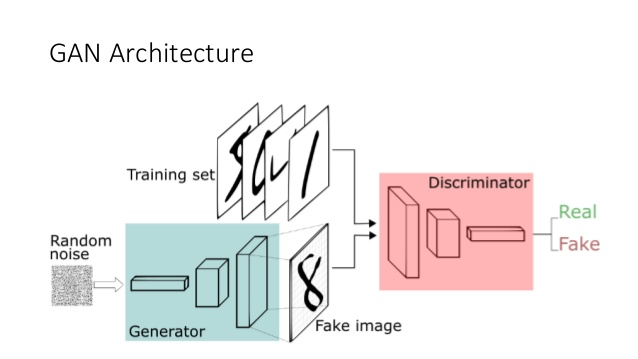
\includegraphics[width=9cm]{gan-arch.jpg}
    \caption{Architecture of a GAN}
    \label{fig:gan}
\end{figure}


% current state of the art

Since the advent of GANs in 2014, they have vastly improved and have blown up in the AI research field.
State of the art research in GANs is currently focusing at applications in video and voice data. 


\subsection{\label{sec:applications}Applications}

GANs have been applied to many problems \cite{overviewDocument}.\\
A sampling of some of the problems are listed below. 

\begin{itemize}
    \item Image Generation
    \item Music Generation
    \item Style Transfer
    \item Video Prediction
    \item Super Resolution
    \item Text to Image 
\end{itemize}


\subsection{\label{sec:level2}Deep Convolutional Generative Adversarial Network}

Deep Convolutional Generative Adversarial Networks, DCGAN for short, is an architectural modification on the original GAN, in which the generator and discriminator models are reflections of one another.
The makeup of each network is a multi-layer, deep convolutional neural network. The idea behind this architecture is that by reflecting the network structure between the two, the computational capacities of each network to learn their respective tasks is equal \cite{radford2015unsupervised}.
In doing this, it should stabilize competitive learning between the two agents and result in an smoother learning, avoiding cases of one network dominance.


\subsection{\label{sec:wgan}Wasserstein Generative Adversarial Networks}

Wasserstein Generative Adversarial Networks, or WGANs for short, were an improvement on the vanilla GAN proposed by Martin Arjovsky, et al in 2017 \cite{arjovsky2017wasserstein}.
The motivation behind this work is modifying the task of the discriminator in order to stabilize the training between the networks. 
Instead of having a simple binary classifier that predicts whether an image is real or fake, the discriminator is modified to output the likelihood estimate of the "realness" or "fakeness" of an image.
The theoretical idea is that this continuous estimation incentivizes the generator to minimize the distance between the distribution of its generated images and the real images more than the standard discriminator design.
Empirically, this design has shown greater results over the standard GAN architecture in terms of training and architecture stability, as well as being more robust to hyper-parameter configurations.

\section{\label{sec:goals}Goals}

% project overview... what we are doing

This project applies three different GAN architectures to generating handwritten images from the MNIST dataset. 
We are going to compare: vanilla GANs, DCGANs, and WGANs.
Using the results of the three different architectures we wish to judge the performance based on three performance criteria:

\begin{itemize}
    \item Perceived Quality of Images
    \item Time required to train
    \item Training data required
\end{itemize}{}

% MNIST data set

The Modified National Institute of Standards and Technology database (MNIST database) is a dataset comprising of seventy thousand handwritten digits.
Sixty thousand of those images are partitioned for training and the remaining ten thousand are left for testing and validation.
We are using the MNIST dataset because it is the de facto standard when it comes to machine learning on images. 


\subsection{\label{sec:researchQuestions}Research Questions}

\begin{itemize}
    \item Which GAN architecture performs best on the MNIST dataset?
    \item What are the quantitative differences between these architectures in terms of stability of training, and quality of the results? 
    \item How does required training time and convergence rate differ between GAN architectures?
\end{itemize}


% ------------------------------------------------ Implementation -----
\section{\label{sec:implementation}Implementation}
% go over how each algorithm was implemented,
% possibly link to github with code

We implemented each GAN variety using PyTorch. PyTorch is an open source machine learning framework. This framework was used due to its popularity in the field and ease of use\cite{pytorch}. Our python implementation can be found on Github in a repository created for this class titled "jrtechs/CSCI-431-final-GANS"\footnote{\url{https://github.com/jrtechs/CSCI-431-final-GANs}}.


\subsection{\label{sec:impVanilla}Vanilla Generative Adversarial Network}
% section covering basic GAN implementation

Using boilerplate PyTorch code we implemented a basic GAN that uses a generator and discriminator using simple neural networks. We used a Binary Cross Entropy (BCE) Loss function for the adversarial algorithm \cite{generalDeepLearning}. 
The arching idea of a basic GAN can be observed in figure \ref{fig:gan}.


\subsection{\label{sec:impDCGAN}Deep Generative Adversarial Network}
% section covering code used to run DCGAN

The code to actually run the DCGAN is identical to the code required to run the regular GAN. The key difference is that we use different types of neural networks in both implementations. In the GAN we just used a normal neural network, but, in the DCGAN we used convolutional neural networks where the generator mirrored the discriminator.


\subsection{\label{sec:impWGAN}Wasserstein Generative Adversarial Network}
% section covering WGAN code

The WGAN implementation was nearly identical to the normal GAN implementation but, the loss function was changed to be the Wasserstein distance. The key benefit of this is that the loss functions that we are trying to optimize now correlatie to image quality. 


%---------------------------------------------- end implementation

%---------------------------------------------- experiment --------------
\section{\label{sec:exp}Experiments}
% goes over the tests ran in the experiment

This section goes over in depth the experiments ran in this project and the results produced from them.


\subsection{\label{sec:dataSet}Data Set}
% describe the mnist data set

The MNIST database of handwritten digits was used to test the GAN algorithms. The MNIST dataset comprises of seventy thousand handwritten digits already partitioned into a training and test set. The Training set contains sixty thousand images and ten thousand images are in the test set. This dataset was collected by using approximately 250 writers. Note: the writers in the training and test sets were disjoint from each other.

The MNIST dataset was selected because it is widely used in the field of computer vision and AI. Its popularity makes it an ideal dataset because we can compare our results with the work of other people. Since it is a large set that was used in prior papers, we also know that we could get a really good confidence score if we were solely creating a classifier. However, in this project we will be generating a discriminator and generator on the mnist set. Never-less, the dataset has proven by other researchers to be sufficient for use in neural networks. This  data is ideal to be used because all images are of fixed size of 20x20 and images have already been normalized. 

The data we used was downloaded from Yann LeCun's website \footnote{\url{http://yann.lecun.com/exdb/mnist/}}.


\subsection{\label{sec:expQuality}Quality}
% simple test where we show our best outputs from each gan

In this experiment we aimed to test the quality of the images produced. In this test we had the GANS generate hand written digits. After scrambling which GAN produced which image, we asked a test participant to rank each image on a scale of 1-10 on how it looks. Ten would indicate that it looked like a human drew this digit and a one would indicate that the image looks bad. After all the data was collected we compared which GAN architecture had the best perceived quality from the participant. 




\subsection{\label{sec:expTime}Training}
% time for each generation? Sorta wishy washy on this one

In this experiment we cut off each GAN after a specif amount of Epochs. We compared the results of the three GAN architectures after different amount of batches. Note: each batch contains 64 images. An epoch is when the algorithm has seen all the data in the set. With the Mnist data set it takes 938 batches to get through all the training data. We sampled after 400 batches, 6000 batches and 
187200 batches --200 Epochs. We did 200 epochs because we wanted to see what the algorithm would look like at its best and we did 400 and 6000 to capture how fast the algorithm learned.

\begin{figure*}[h!]
    \centering
    \subfloat[400 Batches]{{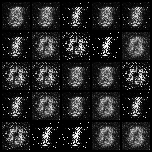
\includegraphics[width=0.3\textwidth]{results/gan/400.png}}}%
    \qquad
    \subfloat[6000 Batches]{{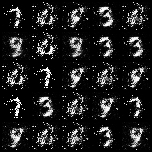
\includegraphics[width=0.3\textwidth]{results/gan/6000.png}}}%
    \qquad
    \subfloat[187200 Batches]{{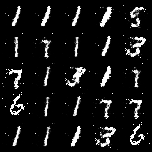
\includegraphics[width=0.3\textwidth]{results/gan/187200.png}}}%
    \caption{GAN Results Sampled at Different Epochs}%
    \label{fig:ganResults}%
\end{figure*}

Looking at figure \ref{fig:ganResults} we see that the normal GAN took some time to train and that it looked pretty bad at 400 and 6000 batches but, started to look pretty good at 200 epochs. 


\begin{figure*}[h!]
    \centering
    \subfloat[400 Batches]{{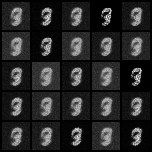
\includegraphics[width=0.3\textwidth]{results/wgan/400.png}}}%
    \qquad
    \subfloat[6000 Batches]{{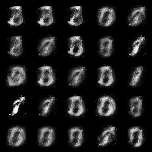
\includegraphics[width=0.3\textwidth]{results/wgan/6000.png}}}%
    \qquad
    \subfloat[187200 Batches]{{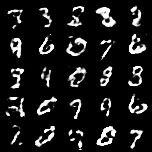
\includegraphics[width=0.3\textwidth]{results/wgan/187200.png}}}%
    \caption{WGAN Results Sampled at Different Epochs}%
    \label{fig:wganResults}%
\end{figure*}

Looking at figure \ref{fig:wganResults} we can see that the results from 400 and 6000 batches were pretty bad but, the results after 200 epochs look remarkably good.

\begin{figure*}[h!]
    \centering
    \subfloat[400 Batches]{{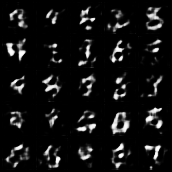
\includegraphics[width=0.3\textwidth]{results/dcgan/400.png}}}%
    \qquad
    \subfloat[6000 Batches]{{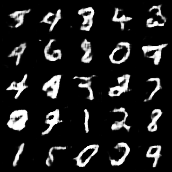
\includegraphics[width=0.3\textwidth]{results/dcgan/6000.png}}}%
    \qquad
    \subfloat[187200 Batches]{{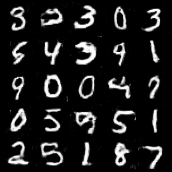
\includegraphics[width=0.3\textwidth]{results/dcgan/187200.png}}}%
    \caption{DCGAN Results Sampled at Different Epochs}%
    \label{fig:dcganResults}%
\end{figure*}

Looking at figure \ref{fig:dcganResults} we notice that training happened remarkably fast. Compared to figure \ref{fig:wganResults} and figure \ref{fig:ganResults} we can observe that the results after 6000 batches looked better than the other two algorithms did after 200 epochs-- 187200 batches. The results of the DCGAN after 200 epochs look remarkable and would easily be passed as human written hand written digets. 

\subsection{\label{sec:expData}Quantity of Training Data}
% vary the amount of training data available to the gans

In this experiment we compare how the GAN algorithms run at different levels of training data from the MNIST set. We compare the GANS using the full training set, half the training set, and an eighth of the dataset. Each algorithm was given 25 epochs to run. 

TODO: run experement


%---------------------------------------- end experiment ----------------


% TODO we might a dedicated results section


\section{\label{sec:exp}Conclusions}
% high level conclusion of results and future work

This project is a useful survey and comparison of three popular GAN architectures. Based on the results we can conclude that....

Future work for this project would entail researching more GAN architectures like Conditional GANS (CGANS), Least Square GANs (LSGAN), Auxiliary Classifier GAN (ACGAN), and Info GANS (infoGAN) \cite{cGAN, lsgan, acgan, infogan},. Another avenue of research would be to examine how the results of our experiments on the MNIST dataset hold up against different data-sets. 

Since this is such a new algorithm in the field of Artificial intelligence, people are still actively doing a ton of research in GANs pushing them at the forefront of cutting edge. As GANs become more widely used in the public and private sector, we are sure to see a lot more research into the applications of GANs.

\section{Acknowledgment}

This was submitted as a RIT CSCI-431 project for professor Sorkunlu's class. Latex files used to generate this report can be found on a Github page created specifically for this project \footnote{\url{https://github.com/jrtechs/computer-vision-GANs-paper}}. 



% bibliography via bibtex
\bibliographystyle{ACM-Reference-Format}
\bibliography{ref}


\end{document}
%
% ****** End of file proposal.tex ******
